\documentclass{article}
% translate with >> pdflatex -shell-escape <file>

% This file is an extract of the PGFPLOTS manual, copyright by Christian Feuersaenger.
% 
% Feel free to use it as long as you cite the pgfplots manual properly.
%
% See
%   http://pgfplots.sourceforge.net/pgfplots.pdf
% for the complete manual.
%
% Any required input files (for <plot table> or <plot file> or the table package) can be downloaded
% at
% http://www.ctan.org/tex-archive/graphics/pgf/contrib/pgfplots/doc/latex/
% and
% http://www.ctan.org/tex-archive/graphics/pgf/contrib/pgfplots/doc/latex/plotdata/

\usepackage{graphics}
\usepackage{pgfplots}
\pgfplotsset{compat=newest}

\pagestyle{empty}
\usepackage{pgfplotstable}
\usepgfplotslibrary{fillbetween}
\pgfrealjobname{survey}
\begin{document}
\beginpgfgraphicnamed{asd}
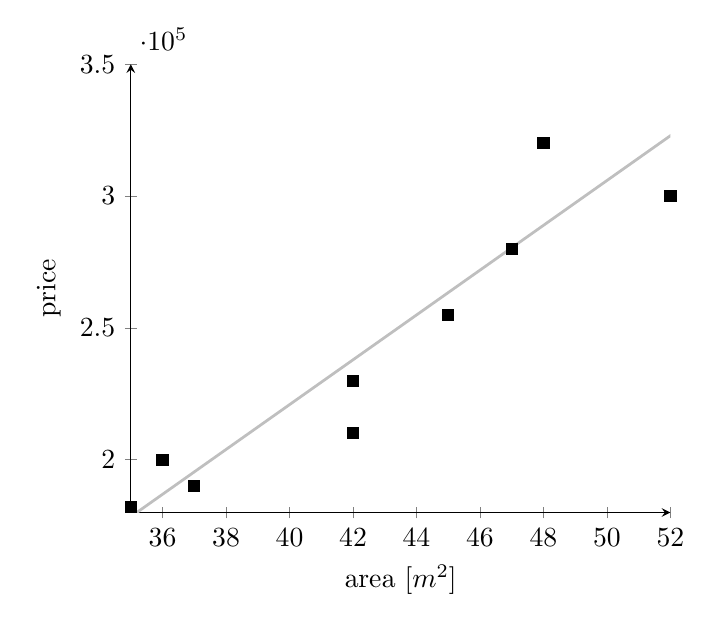
\begin{tikzpicture}
	\begin{axis} [   
    axis y line = left,
    axis x line = bottom,
    domain      = -1.2:4.2,
    xmin = 35, xmax = 52,
    ymin = 180000, ymax = 350000,
		xlabel={area $[{m}^2]$},
	ylabel={price}
	]
	\addplot [only marks, black, mark=square*] table {% plot X versus Y. This is original data.
		X Y
		35 182000
		36 200000
		37 190000
		42 210000
		42 230000
		45 255000
		47 280000
		48 320000
		52 300000
		53 350000
		
	};
	\addplot [name path=line, lightgray,no markers, line width=1pt] table[
		y={create col/linear regression={y=Y}}] % compute a linear regression from the input table
	{
		X Y
		35 180000
		35 200000
		37 190000
		42 210000
		42 230000
		45 255000
		47 280000
		48 320000
		52 300000
		53 350000
	};
	%\xdef\slope{\pgfplotstableregressiona} %<-- might be handy occasionally
	%\addlegendentry{$y(x)$}
	%\addlegendentry{% 
	%	$\pgfmathprintnumber{\pgfplotstableregressiona} \cdot x  
	%	\pgfmathprintnumber[print sign]{\pgfplotstableregressionb}$}
	\end{axis}
\end{tikzpicture}
\endpgfgraphicnamed
\end{document}

